% Options for packages loaded elsewhere
\PassOptionsToPackage{unicode}{hyperref}
\PassOptionsToPackage{hyphens}{url}
\PassOptionsToPackage{dvipsnames,svgnames,x11names}{xcolor}
%
\documentclass[
  letterpaper,
  DIV=11,
  numbers=noendperiod]{scrartcl}

\usepackage{amsmath,amssymb}
\usepackage{iftex}
\ifPDFTeX
  \usepackage[T1]{fontenc}
  \usepackage[utf8]{inputenc}
  \usepackage{textcomp} % provide euro and other symbols
\else % if luatex or xetex
  \usepackage{unicode-math}
  \defaultfontfeatures{Scale=MatchLowercase}
  \defaultfontfeatures[\rmfamily]{Ligatures=TeX,Scale=1}
\fi
\usepackage{lmodern}
\ifPDFTeX\else  
    % xetex/luatex font selection
\fi
% Use upquote if available, for straight quotes in verbatim environments
\IfFileExists{upquote.sty}{\usepackage{upquote}}{}
\IfFileExists{microtype.sty}{% use microtype if available
  \usepackage[]{microtype}
  \UseMicrotypeSet[protrusion]{basicmath} % disable protrusion for tt fonts
}{}
\makeatletter
\@ifundefined{KOMAClassName}{% if non-KOMA class
  \IfFileExists{parskip.sty}{%
    \usepackage{parskip}
  }{% else
    \setlength{\parindent}{0pt}
    \setlength{\parskip}{6pt plus 2pt minus 1pt}}
}{% if KOMA class
  \KOMAoptions{parskip=half}}
\makeatother
\usepackage{xcolor}
\setlength{\emergencystretch}{3em} % prevent overfull lines
\setcounter{secnumdepth}{-\maxdimen} % remove section numbering
% Make \paragraph and \subparagraph free-standing
\ifx\paragraph\undefined\else
  \let\oldparagraph\paragraph
  \renewcommand{\paragraph}[1]{\oldparagraph{#1}\mbox{}}
\fi
\ifx\subparagraph\undefined\else
  \let\oldsubparagraph\subparagraph
  \renewcommand{\subparagraph}[1]{\oldsubparagraph{#1}\mbox{}}
\fi

\usepackage{color}
\usepackage{fancyvrb}
\newcommand{\VerbBar}{|}
\newcommand{\VERB}{\Verb[commandchars=\\\{\}]}
\DefineVerbatimEnvironment{Highlighting}{Verbatim}{commandchars=\\\{\}}
% Add ',fontsize=\small' for more characters per line
\usepackage{framed}
\definecolor{shadecolor}{RGB}{241,243,245}
\newenvironment{Shaded}{\begin{snugshade}}{\end{snugshade}}
\newcommand{\AlertTok}[1]{\textcolor[rgb]{0.68,0.00,0.00}{#1}}
\newcommand{\AnnotationTok}[1]{\textcolor[rgb]{0.37,0.37,0.37}{#1}}
\newcommand{\AttributeTok}[1]{\textcolor[rgb]{0.40,0.45,0.13}{#1}}
\newcommand{\BaseNTok}[1]{\textcolor[rgb]{0.68,0.00,0.00}{#1}}
\newcommand{\BuiltInTok}[1]{\textcolor[rgb]{0.00,0.23,0.31}{#1}}
\newcommand{\CharTok}[1]{\textcolor[rgb]{0.13,0.47,0.30}{#1}}
\newcommand{\CommentTok}[1]{\textcolor[rgb]{0.37,0.37,0.37}{#1}}
\newcommand{\CommentVarTok}[1]{\textcolor[rgb]{0.37,0.37,0.37}{\textit{#1}}}
\newcommand{\ConstantTok}[1]{\textcolor[rgb]{0.56,0.35,0.01}{#1}}
\newcommand{\ControlFlowTok}[1]{\textcolor[rgb]{0.00,0.23,0.31}{#1}}
\newcommand{\DataTypeTok}[1]{\textcolor[rgb]{0.68,0.00,0.00}{#1}}
\newcommand{\DecValTok}[1]{\textcolor[rgb]{0.68,0.00,0.00}{#1}}
\newcommand{\DocumentationTok}[1]{\textcolor[rgb]{0.37,0.37,0.37}{\textit{#1}}}
\newcommand{\ErrorTok}[1]{\textcolor[rgb]{0.68,0.00,0.00}{#1}}
\newcommand{\ExtensionTok}[1]{\textcolor[rgb]{0.00,0.23,0.31}{#1}}
\newcommand{\FloatTok}[1]{\textcolor[rgb]{0.68,0.00,0.00}{#1}}
\newcommand{\FunctionTok}[1]{\textcolor[rgb]{0.28,0.35,0.67}{#1}}
\newcommand{\ImportTok}[1]{\textcolor[rgb]{0.00,0.46,0.62}{#1}}
\newcommand{\InformationTok}[1]{\textcolor[rgb]{0.37,0.37,0.37}{#1}}
\newcommand{\KeywordTok}[1]{\textcolor[rgb]{0.00,0.23,0.31}{#1}}
\newcommand{\NormalTok}[1]{\textcolor[rgb]{0.00,0.23,0.31}{#1}}
\newcommand{\OperatorTok}[1]{\textcolor[rgb]{0.37,0.37,0.37}{#1}}
\newcommand{\OtherTok}[1]{\textcolor[rgb]{0.00,0.23,0.31}{#1}}
\newcommand{\PreprocessorTok}[1]{\textcolor[rgb]{0.68,0.00,0.00}{#1}}
\newcommand{\RegionMarkerTok}[1]{\textcolor[rgb]{0.00,0.23,0.31}{#1}}
\newcommand{\SpecialCharTok}[1]{\textcolor[rgb]{0.37,0.37,0.37}{#1}}
\newcommand{\SpecialStringTok}[1]{\textcolor[rgb]{0.13,0.47,0.30}{#1}}
\newcommand{\StringTok}[1]{\textcolor[rgb]{0.13,0.47,0.30}{#1}}
\newcommand{\VariableTok}[1]{\textcolor[rgb]{0.07,0.07,0.07}{#1}}
\newcommand{\VerbatimStringTok}[1]{\textcolor[rgb]{0.13,0.47,0.30}{#1}}
\newcommand{\WarningTok}[1]{\textcolor[rgb]{0.37,0.37,0.37}{\textit{#1}}}

\providecommand{\tightlist}{%
  \setlength{\itemsep}{0pt}\setlength{\parskip}{0pt}}\usepackage{longtable,booktabs,array}
\usepackage{calc} % for calculating minipage widths
% Correct order of tables after \paragraph or \subparagraph
\usepackage{etoolbox}
\makeatletter
\patchcmd\longtable{\par}{\if@noskipsec\mbox{}\fi\par}{}{}
\makeatother
% Allow footnotes in longtable head/foot
\IfFileExists{footnotehyper.sty}{\usepackage{footnotehyper}}{\usepackage{footnote}}
\makesavenoteenv{longtable}
\usepackage{graphicx}
\makeatletter
\def\maxwidth{\ifdim\Gin@nat@width>\linewidth\linewidth\else\Gin@nat@width\fi}
\def\maxheight{\ifdim\Gin@nat@height>\textheight\textheight\else\Gin@nat@height\fi}
\makeatother
% Scale images if necessary, so that they will not overflow the page
% margins by default, and it is still possible to overwrite the defaults
% using explicit options in \includegraphics[width, height, ...]{}
\setkeys{Gin}{width=\maxwidth,height=\maxheight,keepaspectratio}
% Set default figure placement to htbp
\makeatletter
\def\fps@figure{htbp}
\makeatother

\KOMAoption{captions}{tableheading}
\makeatletter
\@ifpackageloaded{caption}{}{\usepackage{caption}}
\AtBeginDocument{%
\ifdefined\contentsname
  \renewcommand*\contentsname{Table of contents}
\else
  \newcommand\contentsname{Table of contents}
\fi
\ifdefined\listfigurename
  \renewcommand*\listfigurename{List of Figures}
\else
  \newcommand\listfigurename{List of Figures}
\fi
\ifdefined\listtablename
  \renewcommand*\listtablename{List of Tables}
\else
  \newcommand\listtablename{List of Tables}
\fi
\ifdefined\figurename
  \renewcommand*\figurename{Figure}
\else
  \newcommand\figurename{Figure}
\fi
\ifdefined\tablename
  \renewcommand*\tablename{Table}
\else
  \newcommand\tablename{Table}
\fi
}
\@ifpackageloaded{float}{}{\usepackage{float}}
\floatstyle{ruled}
\@ifundefined{c@chapter}{\newfloat{codelisting}{h}{lop}}{\newfloat{codelisting}{h}{lop}[chapter]}
\floatname{codelisting}{Listing}
\newcommand*\listoflistings{\listof{codelisting}{List of Listings}}
\makeatother
\makeatletter
\makeatother
\makeatletter
\@ifpackageloaded{caption}{}{\usepackage{caption}}
\@ifpackageloaded{subcaption}{}{\usepackage{subcaption}}
\makeatother
\ifLuaTeX
  \usepackage{selnolig}  % disable illegal ligatures
\fi
\usepackage{bookmark}

\IfFileExists{xurl.sty}{\usepackage{xurl}}{} % add URL line breaks if available
\urlstyle{same} % disable monospaced font for URLs
\hypersetup{
  pdftitle={Class11: Genomic Informatics},
  pdfauthor={Siyu Xie (PID: A16438448)},
  colorlinks=true,
  linkcolor={blue},
  filecolor={Maroon},
  citecolor={Blue},
  urlcolor={Blue},
  pdfcreator={LaTeX via pandoc}}

\title{Class11: Genomic Informatics}
\author{Siyu Xie (PID: A16438448)}
\date{}

\begin{document}
\maketitle

\renewcommand*\contentsname{Table of contents}
{
\hypersetup{linkcolor=}
\setcounter{tocdepth}{3}
\tableofcontents
}
\section{Section 1. Proportion of G\textbar G in MXL
population}\label{section-1.-proportion-of-gg-in-mxl-population}

Here we read this CSV file

\begin{Shaded}
\begin{Highlighting}[]
\NormalTok{MXL }\OtherTok{\textless{}{-}} \FunctionTok{read.csv}\NormalTok{(}\StringTok{"373531{-}SampleGenotypes{-}Homo\_sapiens\_Variation\_Sample\_rs8067378.csv"}\NormalTok{)}
\FunctionTok{head}\NormalTok{(MXL)}
\end{Highlighting}
\end{Shaded}

\begin{verbatim}
  Sample..Male.Female.Unknown. Genotype..forward.strand. Population.s. Father
1                  NA19648 (F)                       A|A ALL, AMR, MXL      -
2                  NA19649 (M)                       G|G ALL, AMR, MXL      -
3                  NA19651 (F)                       A|A ALL, AMR, MXL      -
4                  NA19652 (M)                       G|G ALL, AMR, MXL      -
5                  NA19654 (F)                       G|G ALL, AMR, MXL      -
6                  NA19655 (M)                       A|G ALL, AMR, MXL      -
  Mother
1      -
2      -
3      -
4      -
5      -
6      -
\end{verbatim}

\begin{Shaded}
\begin{Highlighting}[]
\NormalTok{MXL}\SpecialCharTok{$}\NormalTok{Genotype..forward.strand.}
\end{Highlighting}
\end{Shaded}

\begin{verbatim}
 [1] "A|A" "G|G" "A|A" "G|G" "G|G" "A|G" "A|G" "A|A" "A|G" "A|A" "G|A" "A|A"
[13] "A|A" "G|G" "A|A" "A|G" "A|G" "A|G" "A|G" "G|A" "A|G" "G|G" "G|G" "G|A"
[25] "G|G" "A|G" "A|A" "A|A" "A|G" "A|A" "A|G" "G|A" "G|G" "A|A" "A|A" "A|A"
[37] "G|A" "A|G" "A|G" "A|G" "A|A" "G|A" "A|G" "G|A" "G|A" "A|A" "A|A" "A|G"
[49] "A|A" "A|A" "A|G" "A|G" "A|A" "G|A" "A|A" "G|A" "A|G" "A|A" "G|A" "A|G"
[61] "G|G" "A|A" "G|A" "A|G"
\end{verbatim}

\begin{Shaded}
\begin{Highlighting}[]
\FunctionTok{table}\NormalTok{(MXL}\SpecialCharTok{$}\NormalTok{Genotype..forward.strand.)}
\end{Highlighting}
\end{Shaded}

\begin{verbatim}

A|A A|G G|A G|G 
 22  21  12   9 
\end{verbatim}

\begin{Shaded}
\begin{Highlighting}[]
\FunctionTok{table}\NormalTok{(MXL}\SpecialCharTok{$}\NormalTok{Genotype..forward.strand.)}\SpecialCharTok{/}\FunctionTok{nrow}\NormalTok{(MXL)}\SpecialCharTok{*}\DecValTok{100}
\end{Highlighting}
\end{Shaded}

\begin{verbatim}

    A|A     A|G     G|A     G|G 
34.3750 32.8125 18.7500 14.0625 
\end{verbatim}

Now lets look at a different population.

\begin{Shaded}
\begin{Highlighting}[]
\NormalTok{GBR }\OtherTok{\textless{}{-}} \FunctionTok{read.csv}\NormalTok{(}\StringTok{"373522{-}SampleGenotypes{-}Homo\_sapiens\_Variation\_Sample\_rs8067378.csv"}\NormalTok{)}
\end{Highlighting}
\end{Shaded}

\begin{Shaded}
\begin{Highlighting}[]
\FunctionTok{head}\NormalTok{(GBR)}
\end{Highlighting}
\end{Shaded}

\begin{verbatim}
  Sample..Male.Female.Unknown. Genotype..forward.strand. Population.s. Father
1                  HG00096 (M)                       A|A ALL, EUR, GBR      -
2                  HG00097 (F)                       G|A ALL, EUR, GBR      -
3                  HG00099 (F)                       G|G ALL, EUR, GBR      -
4                  HG00100 (F)                       A|A ALL, EUR, GBR      -
5                  HG00101 (M)                       A|A ALL, EUR, GBR      -
6                  HG00102 (F)                       A|A ALL, EUR, GBR      -
  Mother
1      -
2      -
3      -
4      -
5      -
6      -
\end{verbatim}

Find proportion of G\textbar G of GBR

\begin{Shaded}
\begin{Highlighting}[]
\FunctionTok{round}\NormalTok{(}\FunctionTok{table}\NormalTok{(GBR}\SpecialCharTok{$}\NormalTok{Genotype..forward.strand.)}\SpecialCharTok{/}\FunctionTok{nrow}\NormalTok{(GBR)}\SpecialCharTok{*}\DecValTok{100}\NormalTok{,}\DecValTok{2}\NormalTok{)}
\end{Highlighting}
\end{Shaded}

\begin{verbatim}

  A|A   A|G   G|A   G|G 
25.27 18.68 26.37 29.67 
\end{verbatim}

This variant associated with childhood asthma is more frequent in the
GBR than in MXL population.

Lets now dig into this further.

\subsection{Section 4 Population
Analysis}\label{section-4-population-analysis}

One sample is obviously not enough to know what is happening in a
population. You are interested in assessing genetic differences on a
population scale.

So, you processed about \textasciitilde230 samples and did the
normalization on a genome level. Now, you want to find whether there is
any association of the 4 asthma-associated SNPs (rs8067378\ldots) on
ORMDL3 expression.

\begin{quote}
Q13.Read this file into R and determine the sample size for each
genotype and their corresponding median expression levels for each of
these genotypes
\end{quote}

\begin{Shaded}
\begin{Highlighting}[]
\NormalTok{expr }\OtherTok{\textless{}{-}} \FunctionTok{read.table}\NormalTok{(}\StringTok{"rs8067378\_ENSG00000172057.6.txt"}\NormalTok{)}
\FunctionTok{head}\NormalTok{(expr)}
\end{Highlighting}
\end{Shaded}

\begin{verbatim}
   sample geno      exp
1 HG00367  A/G 28.96038
2 NA20768  A/G 20.24449
3 HG00361  A/A 31.32628
4 HG00135  A/A 34.11169
5 NA18870  G/G 18.25141
6 NA11993  A/A 32.89721
\end{verbatim}

\begin{Shaded}
\begin{Highlighting}[]
\FunctionTok{library}\NormalTok{(dplyr)}
\end{Highlighting}
\end{Shaded}

\begin{verbatim}

Attaching package: 'dplyr'
\end{verbatim}

\begin{verbatim}
The following objects are masked from 'package:stats':

    filter, lag
\end{verbatim}

\begin{verbatim}
The following objects are masked from 'package:base':

    intersect, setdiff, setequal, union
\end{verbatim}

\begin{Shaded}
\begin{Highlighting}[]
\NormalTok{expr }\SpecialCharTok{\%\textgreater{}\%}
  \FunctionTok{group\_by}\NormalTok{(geno) }\SpecialCharTok{\%\textgreater{}\%}
  \FunctionTok{summarize}\NormalTok{(}
    \AttributeTok{sample\_size =} \FunctionTok{n}\NormalTok{ (),}
    \AttributeTok{median\_expression =} \FunctionTok{median}\NormalTok{ (exp, }\AttributeTok{na.rm=}\ConstantTok{TRUE}\NormalTok{)}
\NormalTok{  )}
\end{Highlighting}
\end{Shaded}

\begin{verbatim}
# A tibble: 3 x 3
  geno  sample_size median_expression
  <chr>       <int>             <dbl>
1 A/A           108              31.2
2 A/G           233              25.1
3 G/G           121              20.1
\end{verbatim}

\begin{quote}
Q14. Generate a boxplot with a box per genotype, what could you infer
from the relative expression value between A/A and G/G displayed in this
plot? Does the SNP effect the expression of ORMDL3?
\end{quote}

A: the median level of expression for A\textbar A is significantly
higher than G\textbar G, meaning the SNP does affect the expression of
ORMDL3.

\begin{Shaded}
\begin{Highlighting}[]
\FunctionTok{library}\NormalTok{(ggplot2)}
\end{Highlighting}
\end{Shaded}

\begin{Shaded}
\begin{Highlighting}[]
\FunctionTok{ggplot}\NormalTok{(expr) }\SpecialCharTok{+}
  \FunctionTok{aes}\NormalTok{(}\AttributeTok{x =}\NormalTok{ geno, }\AttributeTok{y =}\NormalTok{ exp, }\AttributeTok{fill =}\NormalTok{ geno)}\SpecialCharTok{+}
  \FunctionTok{geom\_boxplot}\NormalTok{(}\AttributeTok{notch =} \ConstantTok{TRUE}\NormalTok{)}
\end{Highlighting}
\end{Shaded}

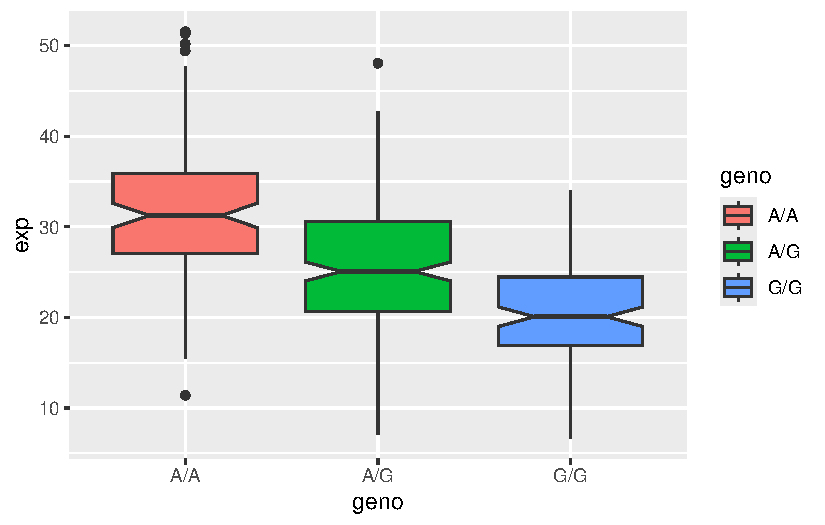
\includegraphics{./-class11_files/figure-pdf/unnamed-chunk-10-1.pdf}



\end{document}
